\chapter{Learning the Optimal Speed Profile}
\label{chapter5}

The iterative learning algorithms presented in Chapter 4 can help an autonomous vehicle follow a desired trajectory more precisely over 
several laps of driving. However, the ILC algorithms do not alter the trajectory itself, only the input signals that attempt
to track the trajectory. This will not be sufficient at the limits of handling. 
Consider Fig.~{\ref{fig:expErrors}, reprinted below. The speed profile was generated assuming a tire-road friction value of $\mu = 0.94$.
Since peak vehicle acceleration is given by $\mu g$, this corresponds to maximum lateral and longitudinal acceleration values of 9.4 $\mathrm{m/s^2}$.
While this is a reasonable assumption overall, there are several parts on the track where the vehicle exceeds the available friction and begins
to understeer. Region \circled{2} is one example. The tire slip norm $\zeta$ (\ref{eq:zeta}) climbs above one, and as a result, the vehicle begins
to slide off the track, resulting in the large negative tracking error spike in Fig.~{\ref{fig:expErrors2}(b). The vehicle's stability
algorithms (not discussed in this thesis, see \cite{mickthesis}) kick in and slow the vehicle down, which results in the speed tracking
error seen in Fig.~{\ref{fig:expErrors2}(a). In this situation, iterative learning control will be unable to achieve better speed tracking
and lateral tracking performance. The tires are saturated and the car is slowly beginning to careen off the track. Simply steering more
on the next lap will not achieve better tracking performance due to the saturation of the steering actuator. In order to recover, the vehicle must deviate
from the planned trajectory, either by slowing down or by taking a wider radius turn.
 
 \begin{figure}[h!]
\centering
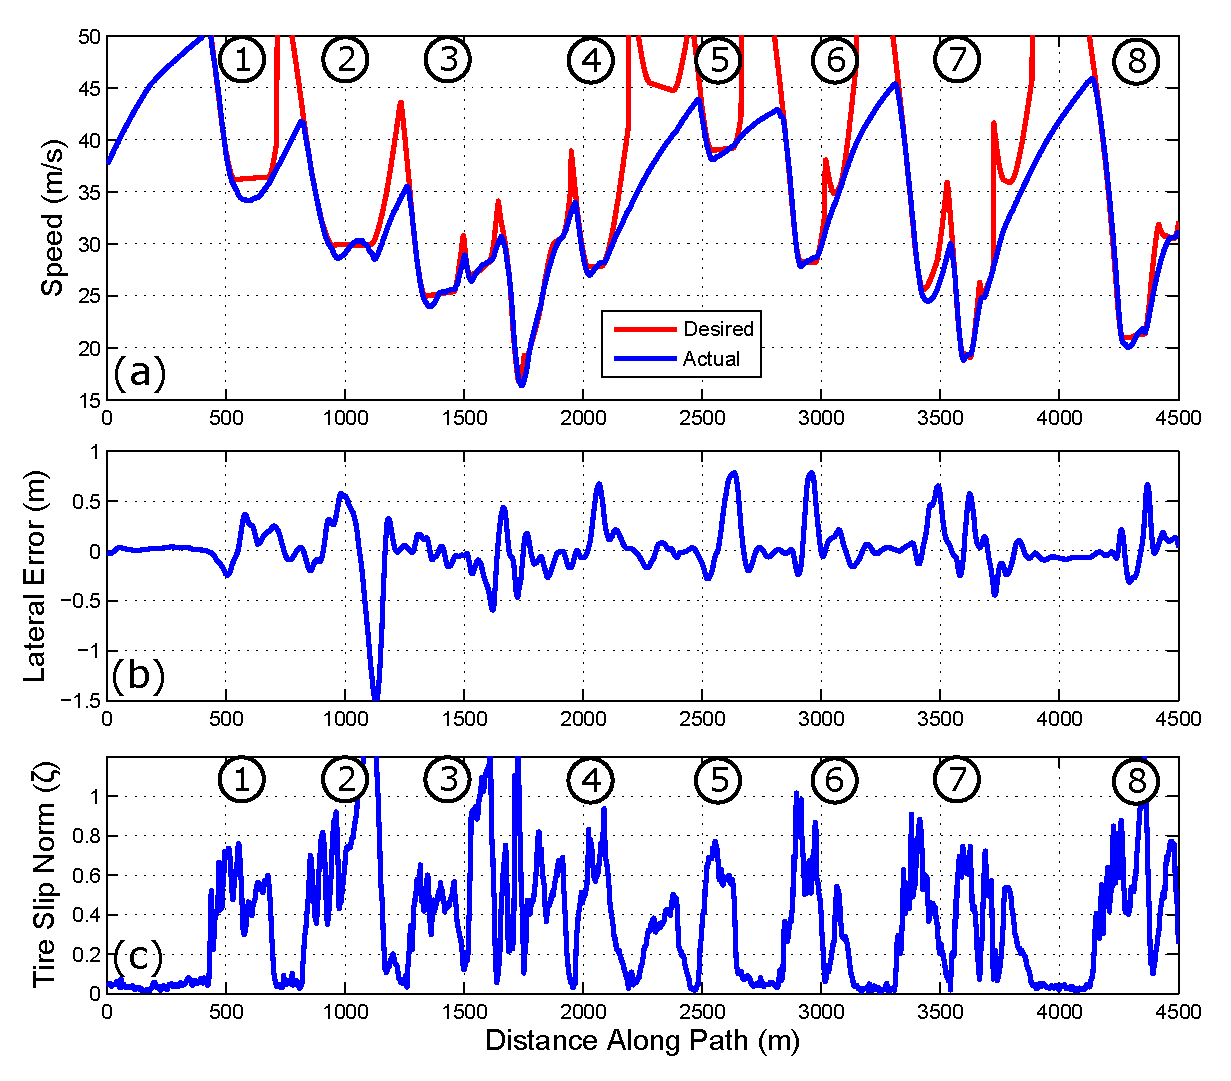
\includegraphics[width=.9\fullwidth]{expErrors.eps}
\caption{Reprint of Fig.~\ref{fig:expErrors}. Controller tracking performance and tire slip norm on a test run at the limits of handling ($\mu =$ 0.95).}
\label{fig:expErrors2}
\end{figure}

\newpage
As another situation, consider region \circled{3}. While the vehicle exceeds the friction limit on the prior section of the track, 
here the vehicle does not appear close to the limits at all, with $\zeta \approx $ 0.6. A professional human driver would feel the vehicle being below the limits
of handling and would increase her speed to decrease the time through the turn. However, ILC is only concerned with trajectory tracking,
and would not raise the speed above the planned trajectory. 

These two situations demonstrate the need for separate algorithms that learn from data in order to modify the desired \textit{trajectory itself}
as opposed to just the control signals that attempt to track it. Trajectory modification algorithms previously investigated in
the literature have focused on modifying the \textit{lateral} trajectory by altering the curvature profile as the vehicle understeers
or oversteers. For example, Theodosis presented 
an algorithm to gradually widen the radius of a turn in response to a detected understeer \cite{paulthesis}. The algorithm was validated
experimentally, but assumed sufficient availability of road width. Klomp and Gordon also developed a strategy for recovering from
vehicle understeer by solving for an optimal emergency braking profile to minimize deviation from the desired path \cite{klomp}. Funke et al.~\cite{funkeIV} presented a model predictive control (MPC)
approach that generally aimed
to follow a planned vehicle trajectory at the limits. However, if the vehicle was at risk of understeering or oversteering, the MPC algorithm
would deviate laterally from the planned trajectory in order to maintain stability of the vehicle without driving off the road. 

This chapter presents an algorithm that takes a different approach. Instead of modifying the curvature profile, an A*
search algorithm is presented
that modifies portions of the \textit{velocity} profile to be more conservative if a stability violation is encountered on a prior lap. This is accomplished by
generalizing the speed profile such that each part of the track can be driven with a different assumed value of friction $\mu$ and therefore a different maximum
acceleration. Since this dissertation is concerned with
racing as well, the algorithm also modifies the velocity profile to be more aggressive if the tires are not being driven at the limits. Finally,
instead of acting as a stability controller that modifies the trajectory in real time, the presented algorithm relies on a previously
implemented controller \cite{mickthesis} for real-time stabilization and focuses on learning the time-optimal friction profile $\mu^\star(s)$ by searching through datasets obtained over multiple laps. 

\section{Effect of Tire Slip Norm on Lap Time}
\label{sec:etu}

Fig.~\ref{fig:t2} shows the complicated effect of driving at different levels of lateral and longitudinal acceleration for region \circled{2} in Fig.~\ref{fig:expErrors2}. Recall that the
speed profile is generated by assuming a global value of tire friction $\mu$, which is directly related to the acceleration norm of
the desired speed profile ($\sqrt{a_x^2 + a_y^2}$) by a factor of \mbox{$g =$ 9.81 $\mathrm{m/s^2}$}. Fig.~\ref{fig:t2}(a) confirms that higher levels
of $\mu$ result in strictly faster speed profiles for the same turn. 

\begin{figure}
\centering
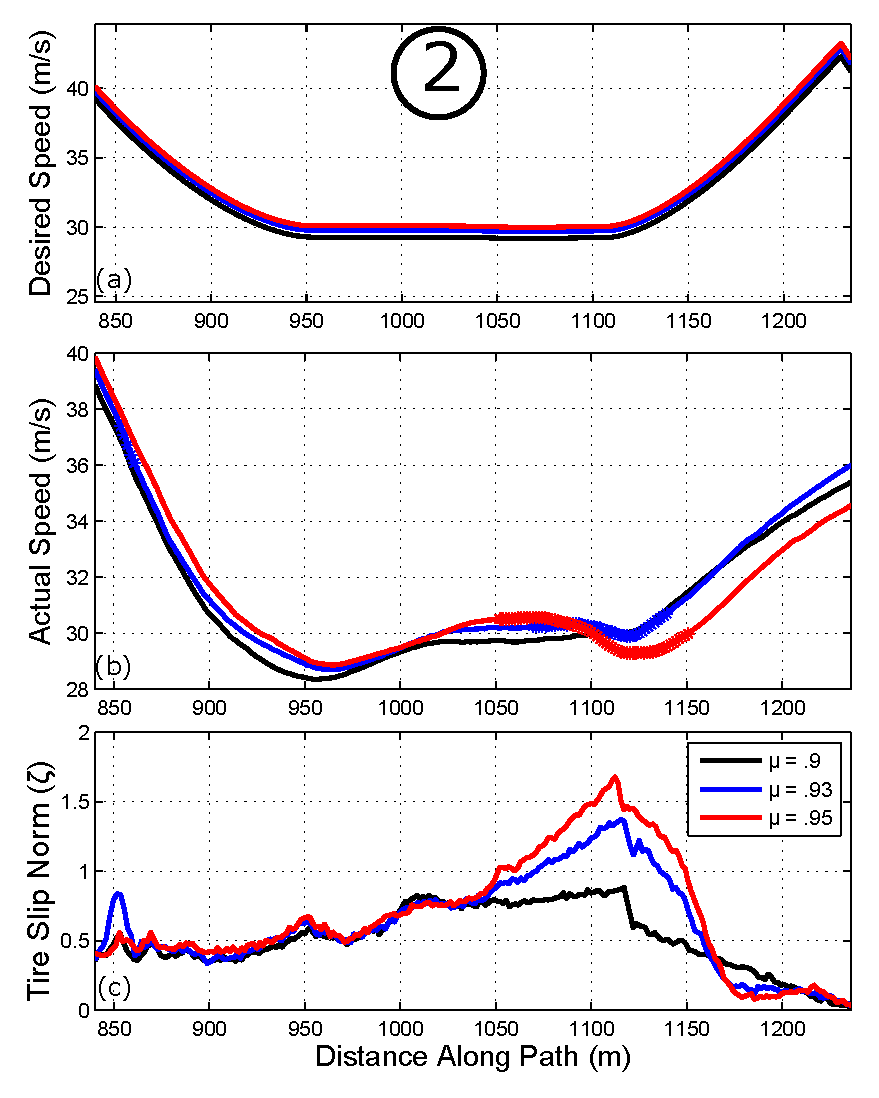
\includegraphics[width=.8\fullwidth]{t2res.eps}
\caption[Desired speed for varying levels of $\mu$ - region 2]{(a) Desired speed for varying levels of $\mu$ (b) Actual speed for varying levels of $\mu$. Asterisks correspond to 
regions where $\zeta > 1$. (c) Tire slip norm for varying levels of $\mu$. }
\label{fig:t2}
\end{figure}

However, selecting a more aggressive value of $\mu$ does not necessarily entail a faster experimental lap time. Consider the actual speeds of the vehicle in
Fig.~\ref{fig:t2}(b) when trying to experimentally follow three different speed profiles. For the case where $\mu = 0.9$, the vehicle completes
the turn without fully utilizing the tire's capability and achieves relatively low velocities. For the extreme case where $\mu = 0.95$, the
vehicle enters the turn at a high speed but then begins to slide as $\zeta = 1.6$. While not shown in the plot, the saturation
is occurring primarily at the front tires, causing an understeer that can cause the car to skid off the track. Completing the lap therefore requires a stabilizing
action from the stability controller to slow the car down and regain control of the vehicle. As a result,
when the vehicle accelerates at the end of the turn, the actual vehicle speed at $\mu = 0.95$ is significantly slower than the case where $\mu = 0.9$!
A final ``just right" value of $\mu = 0.93$ was also tested experimentally for this turn, and while the car does slide a bit at this level of driving (peak $\zeta = 1.3$),
the needed stabilizing action is significantly smaller and the vehicle exits the turn with the highest speed. 

 \begin{figure}[tb]
\centering
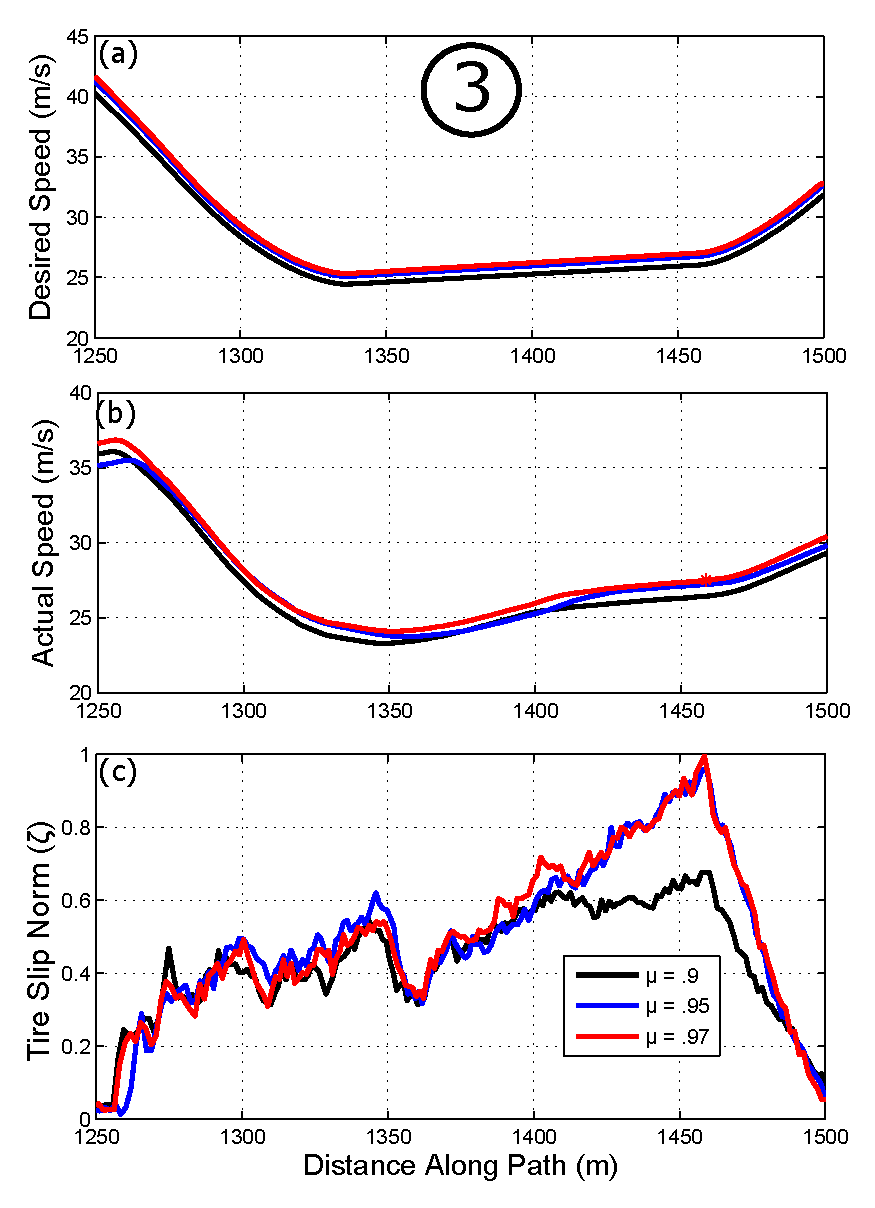
\includegraphics[width=.8\fullwidth]{t3res.eps}
\caption[Desired speed for varying levels of $\mu$ - region 3]{(a) Desired speed for varying levels of $\mu$. (b) Actual speed for varying levels of $\mu$. Asterisks correspond to 
regions where $\zeta > 1$. (c) Tire slip norm for varying levels of $\mu$. }
\label{fig:t3}
\end{figure}

Unfortunately, the best value of $\mu$ is not constant throughout the track. Fig.~\ref{fig:t3} shows the same data plotted for region \circled{3} of the 
Thunderhill Raceway. In this case, even with an atypically high value of 
$\mu = 0.97$, the slip norm of the vehicle tires is relatively low, and the value of $\mu$ that optimizes the completion time for this turn could 
be even larger. 

\section{Naive Method: Greedy Algorithm}
\label{sec:greedy}

Section \ref{sec:etu} shows that to  minimize the overall lap time, there is a need to generalize the speed profile such that different portions of the track can be driven with different
values of $\mu$. In other words, \textbf{the problem is to learn the ``friction profile" $\mu^\star(s)$ along the path that minimizes the experimental vehicle lap time.} 

The simplest approach to finding $\mu(s)$ is a greedy algorithm where a set of experimental data is collected for a variety of different
speed profiles, each corresponding to a different value of $\mu$ and therefore a different acceleration level. The greedy approach is then to discretize
the track into a number of small sections and pick the value of $\mu$ for each section that corresponds to the highest observed experimental velocity.
The final desired velocity profile is then generated using the numerical integration approach presented in \S \ref{sec:VP}. This method does not require a single 
value of friction across the whole track, and generates a smooth velocity profile even when the peak acceleration limits vary from point to point. 

 \begin{figure}[tb]
\centering
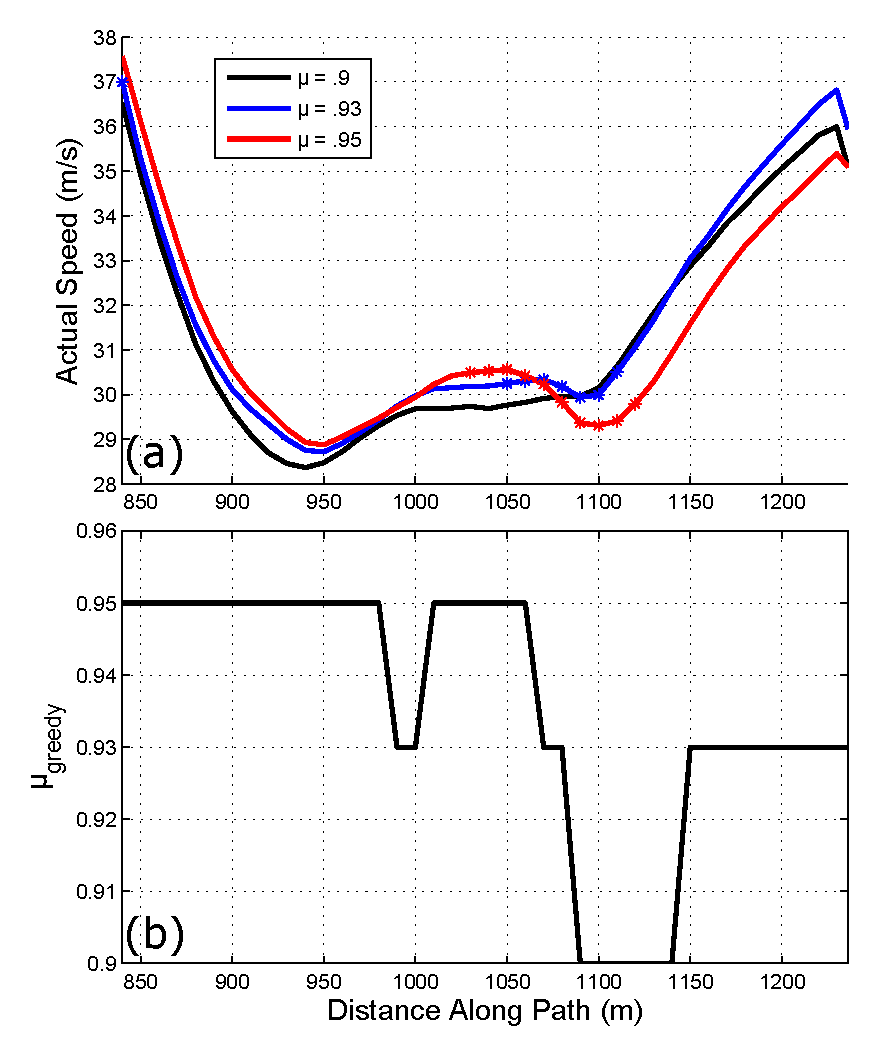
\includegraphics[width=.85\fullwidth]{turn2greedy.eps}
\caption[Greedy algorithm results for region 2.]{(a) Desired speed for varying levels of $\mu$ (b)``Greedy" value of $\mu$ as a function of distance along track. Asterisks denote
region of track where vehicle is understeering.}
\label{fig:t2g}
\end{figure}

A plot showing the results of applying the greedy algorithm for section \circled{2} is shown in Fig.~\ref{fig:t2g}. The flaw in simply
selecting $\mu$ based on the highest speeds is apparent at $s = 1050 \mathrm{m}$. The greedy algorithm suggests the vehicle mostly drive at $\mu$ = 0.95,
but then switch to driving at $\mu = 0.93$ as soon as the vehicle begins to slide. Switching to a less aggressive velocity profile at this
point is impossible to achieve in practice, because the vehicle is already fully sliding and has no control until the vehicle slows down.
As a result, the greedy algorithm fails to capture the hidden cost of a large understeer, which results in a period of time where the speed must
inevitably drop. 

\section{Framing Trajectory Learning as Search \newline Problem}
\label{sec:framingTL}

Given the inadequacy of the greedy algorithm, a more sophisticated approach is necessary to learn $\mu^\star(s)$ from
experimentally observed data. This section frames the desire to find the minimum time $\mu^\star(s)$ as a tree search problem.
Consider discretizing the racing path into $N$ evenly spaced segments. For example, on the Thunderhill Raceway with
$\Delta s = 5 \mathrm{m}$, $\textbf{s} = [0 \hspace{2mm} 5 \hdots s_k \hdots 4495 \hspace{2mm} 4500]$ for $k = 0 \hdots N$, with $N = 901$. For each
path distance $s_k$, there are $M_k$ velocity and $M_k$ tire slip observations from experimental data, each corresponding to a different $\mu$. 
For example, looking at Fig.~\ref{fig:t2}, if $k = 191$, $s_k =  950 \mathrm{m}$, $M_k = 3$, the velocity and slip norm $\zeta$ observations $U_k(\mu)$ and $Z_k(\mu)$ are as follows:

\begin{table}[h]
\begin{center}
\caption{$U_k(\mu)$ and $Z_k(\mu)$ for $k =$ 191}\label{tb:laptimes}
\begin{tabular}{ccc}
$\mu $&$ U_x(m/s) $& $\zeta $\\\hline
0.9 & 28.42 & 0.55\\
0.93& 28.91 & 0.63\\
0.95& 29.14 & 0.66\\\hline
\end{tabular}
\end{center}
\end{table} 
 $M_k$ is not necessarily the same for all $k$ to account for experimental trials that do not cover the full lap. For safety and time
 reasons, some parts of the track will only have experimental data collected at two different friction values, while others may have five or six.

 Nodes of the search tree are then defined as a two-element state tuple, with the first state element being $s_k$ and the second element being the current
 friction coefficient $\mu_k$. Since the car must start from the beginning of the path, the first state has $s_0 = 0$.
 The $M_k$ edges from a given node correspond to actions that the car can take at $s = s_k$. In this case, the ``action" is the next value of $\mu$,
 and the successor states are $(s_{k+1}, \mu_1) ... (s_{k+1}, \mu_{M_k})$. A diagram of the search tree is shown in Fig.~\ref{fig:stree}.

 \newpage
  \begin{figure}[h!]
\centering
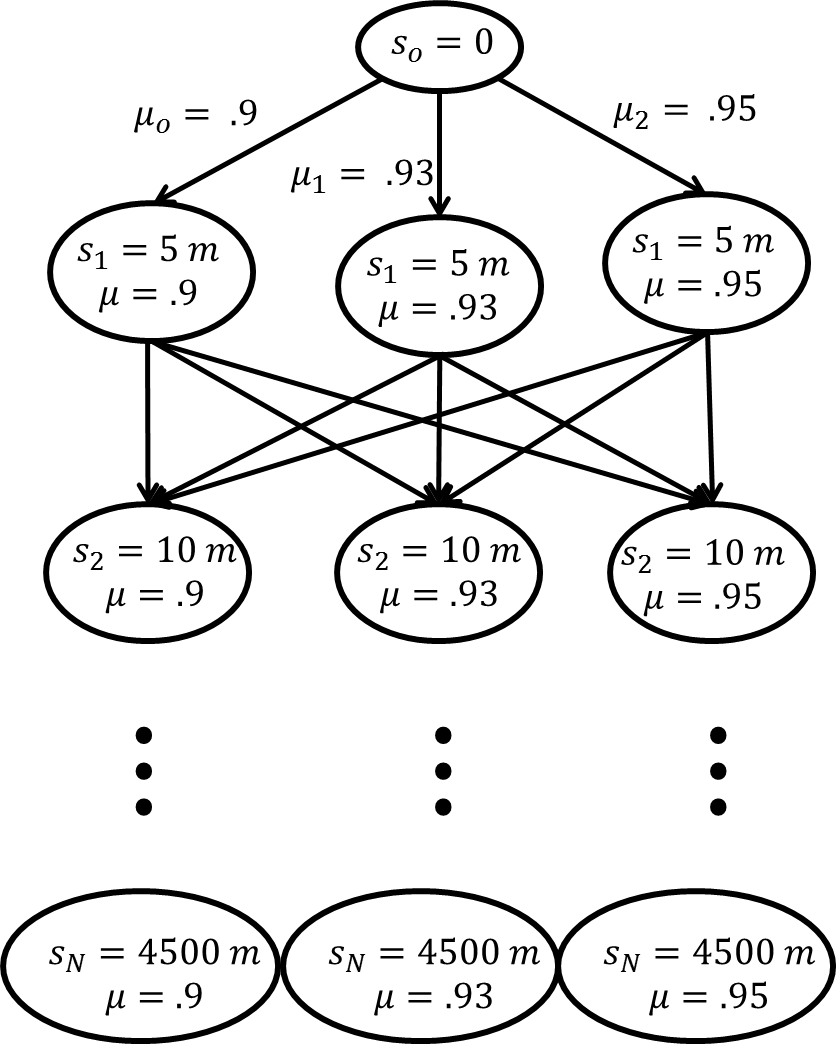
\includegraphics[width=.85\fullwidth]{searchTree.png}
\caption{Sample search tree for Thunderhill race track where there are only 3 experimentally observed full laps at $\mu =$ 0.9, 0.93, 0.95.}
\label{fig:stree}
\end{figure} 
\newpage
 
Each edge is associated with a travel cost $c_t$. The travel cost for a given edge is the amount of time it takes to go from
$s = s_k$ to $s = s_{k+1}$ driving at the friction coefficient $\mu$ associated with that edge. As illustrated in Fig.~\ref{fig:costDiag}, the cost is estimated from the experimentally
observed data assuming linear acceleration between points. The travel cost from node $(s_k, \mu_k)$ to $(s_{k+1}, \mu_{k+1})$ can therefore be expressed mathematically with trapezoidal integration of the straight-line velocity profile:
\begin{align}
c_t(s_k, s_{k+1},\mu_k, \mu_{k+1}) &= \ln \frac{a_x(\Delta s) + U_k(\mu_k)}{a_x} - \ln \frac{U_k(\mu_k)}{a_x} \\
a_x &= \frac{U_{k+1}(\mu_{k+1}) - U_k(\mu_k)}{\Delta s}
\end{align}

 \begin{figure}[tb]
\centering
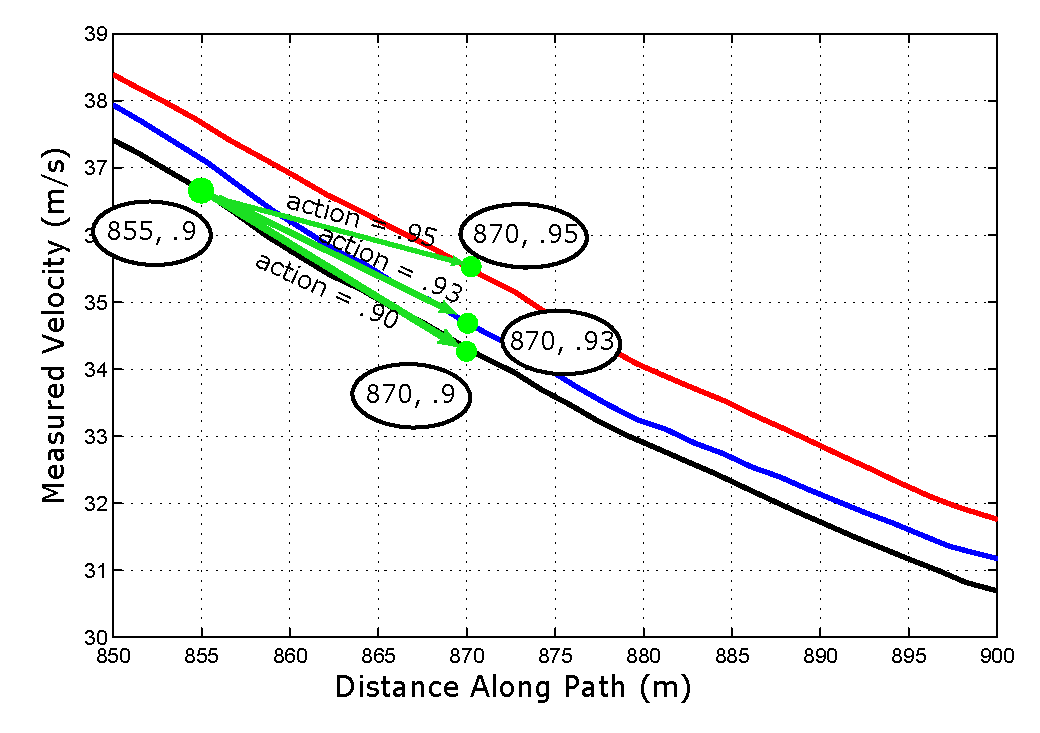
\includegraphics[width=\fullwidth]{costStructure.eps}
\caption[Illustration of travel cost.]{Illustration of travel cost. Current state is (855, 0.9). Assuming $\Delta s$ is 15 meters, cost is time to travel from this node
to one of the three possible successor nodes, depending on the action taken.}
\label{fig:costDiag}
\end{figure} 
\newpage
In addition to the travel cost, there is also a \textit{switching} cost $c_s$ associated with switching to a different value of $\mu$. These
are determined by the observed tire slip norm measurements $Z_k(\mu)$. The switching cost is expressed mathematically as:

\begin{equation}
\label{eq:swCost}
c_s(s_k, s_{k+1},\mu_k, \mu_{k+1}) =\mathds{1}\left(\mu_{k+1} \neq \mu_{k}\right)\left(\lambda  + \infty \times\mathds{1}\left(Z_k(\mu_k) > 1\right) \right)
\end{equation}

Where $\mathds{1}$ is the indicator function. The switching cost function (\ref{eq:swCost}) implies that an action will never
incur a switching cost if the selected value of $\mu$ is unchanged from the previous selection. If the value of $\mu$ does change, there
is a small switching penalty $\lambda$, chosen by trial and error to discourage the search algorithm from changing the friction profile to gain a
trivial decrease in lap time. Additionally, there is a very large (infinite) switching penalty if the search algorithm attempts to change the
friction profile while the vehicle's tires are saturated ($\zeta > 1$). This reflects the physical inability of the car to control its
trajectory while sliding and is what separates the search algorithm from the greedy algorithm. A diagram demonstrating (\ref{eq:swCost})
is shown in Fig.~\ref{fig:swCost}. 

 \begin{figure}[tb]
\centering
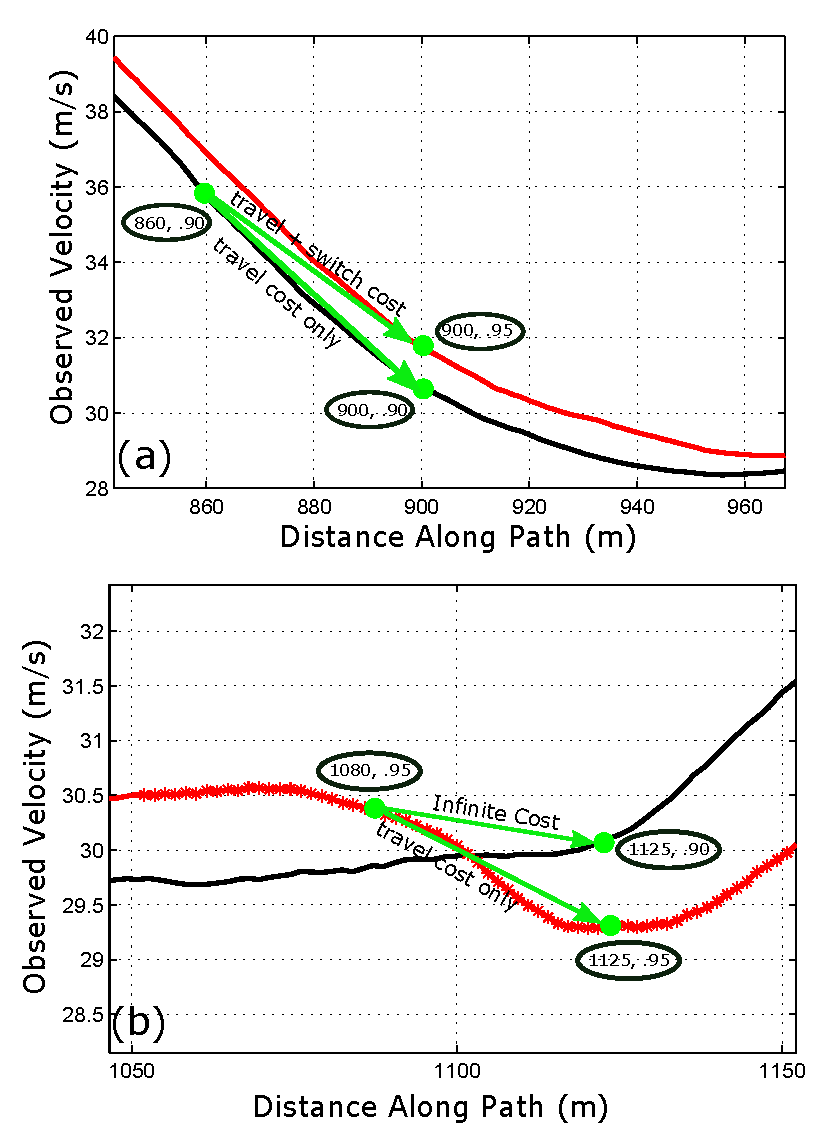
\includegraphics[width=.75\fullwidth]{switchCost.eps}
\caption[Costs when vehicle is and is not sliding.]{(a) Costs when vehicle currently is not sliding. The vehicle can switch to a more aggressive velocity profile, paying a small
switching penalty, or can continue on the current profile. (b) Costs when vehicle is currently sliding. Vehicle has no choice but to continue on current
trajectory. Asterisks denote regions where $\zeta > 1$ and the vehicle is sliding.}
\label{fig:swCost}
\end{figure} 

\section{A* Search Algorithm and Heuristic}
\label{sec:ch5astarheuristic}

Once the tree is mathematically defined in terms of the start state, nodes, edges, and costs, the search problem is to find the sequence
of actions from the start node to any terminal node that minimizes the total cost. In our case, the start state, nodes, edges
and costs were defined in the previous section, and a terminal node is any node at the end of the path (i.e. $k = N$). The sequence
of actions in our case is the friction profile $\mathbf{\mu} = [\mu_1 \hdots \mu_k \hdots \mu_N]$, which determines how
aggressively the vehicle will drive on every part of the track. The total cost is the sum of all individual travel costs $c_t$ and switching costs
$c_s$, and has intuitive units of time. 

Minimum-cost tree spanning algorithms (e.g. breadth-first search, Dijkstra's algorithm, etc.) are a well known subject and a thorough description
can be found in \cite{aibook}. For the purpose of solving this search problem, the A* search algorithm is used. 
Like breadth-first search, the A* algorithm is guaranteed to find the lowest cost path from a start node to a goal node, 
but uses a priority queue data structure to more efficiently explore the search tree. Frontier leaf nodes $n$ being
considered for exploration are ranked according to the following modified cost:

\begin{equation}
f(n) = g(n) + h(n)
\end{equation}
where $g(n)$ is the true cost to go from the start node to node $n$. The function $h(n)$ is a heuristic estimate of the cost to get from node $n$ to any goal state (i.e. to the end of the
path). For A* to be guaranteed to find the shortest path, $h(n)$ must be \textit{admissible}, meaning that $h(n)$ must underestimate the
true cost of getting to the end of the path. 

In our case, we have a very intuitive heuristic function $h(n)$ for the A* implementation. In Sec. \ref{sec:greedy}, the greedy approach
was discussed. Define \newline $\mathbf{U_\mathrm{g}} = [U_\mathrm{g}(1) \hdots U_\mathrm{g}(k) \hdots U_\mathrm{g}(N)]$ to be the highest observed
experimental speed for each index $s_k$. Because we know tracking this greedy profile is physically impossible due to vehicle sliding, time estimates
from this profile will always underestimate the true cost. We therefore define $h(n)$ as follows:

\begin{equation}
\label{eq:heuristic}
h(n) = \int^{s_N}_{s_n} \frac{1}{U_g(s)} ds
\end{equation}
where $s_n$ is the value of $s$ corresponding to node $n$ and $s_N$ is the total length of the track. While (\ref{eq:heuristic}) is an integral equation, it can be solved for the discrete
array $\mathbf{U}_\mathrm{g}$ via trapezoidal numerical integration.

\section{A* Implementation and Results}

Because the A* algorithm relies on experimental observations to learn $\mu^\star(s)$, experimental data was collected over several trials, with
each trial consisting of a speed profile generated with a constant $\mu$ value over the track. The $\mu$ values chosen for
experimental data collection were 0.85, 0.9, 0.92, 0.93, 0.94, 0.95, and 0.97. Ideally, each speed profile would be tested experimentally for a 
full lap at high speed. However, due to safety and time constraints associated with collecting high speed race data, only the speed profiles corresponding to $\mu = 0.92$ and $\mu = 0.94$ were observed
over the whole track. The other speed profiles were only tested on sections of the track. Fig.~\ref{fig:muCoverage} shows the experimental data coverage. 

\begin{table}[h]
\begin{center}
\caption{Search Algorithm Information}\label{tb:astarparams}
\begin{tabular}{lccc}
Parameter & Symbol & Value & Units \\\hline
Track Length       & $L$           &  4500 & $\mathrm{m} $ \\
Discretization Length               & $\Delta s$  & 5 & $\mathrm{m}$\\
Number of Points  & $N$                        & 901 & -\\
Switching Cost          & $\lambda$                        & 0.05   & s\\\hline
CPU Solution Time           &                                  &  70    & s \\
Nodes Explored              &                                  &  6887  & - \\\hline
\end{tabular}
\end{center}
\end{table}

 \begin{figure}[tb]
\centering
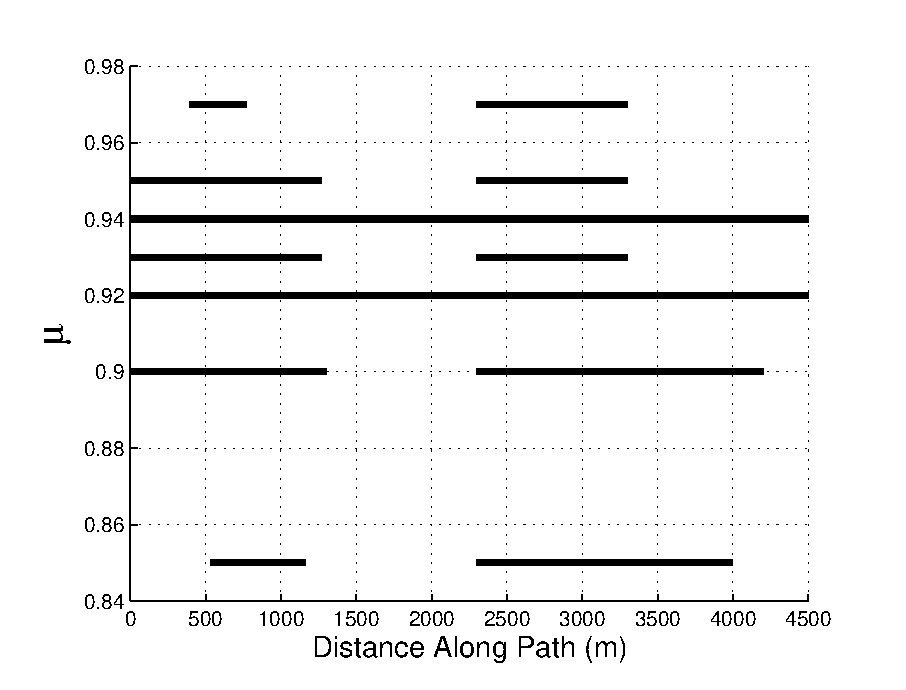
\includegraphics[width=.7\fullwidth]{muCoverage.eps}
\caption[Coverage of experimental data]{Coverage of experimental data. For speed profiles corresponding to $\mu = 0.92$ and $\mu = 0.94$, experimental data of the autonomous race vehicle was observed
over the whole track. For safety and time constraints, the other speed profiles were only tested on sections of the track.}
\label{fig:muCoverage}
\end{figure} 

After collecting the experimental data, the A* algorithm was applied to learn the optimal friction profile $\mu^\star(s)$. Parameters for the algorithm
are shown in Table~\ref{tb:astarparams}. To interface more efficiently with experimental data files, the search algorithm was implemented in MATLAB using
custom code instead of a standard search algorithm library. The entire search process took approximately 70 seconds on a core i7 laptop machine,
exploring 6887 nodes in the process. However, since MATLAB is not designed for computational efficiency in tree-based search algorithms, a C++ implementation would likely
be several orders of magnitude faster. 

 The resulting $\mu^\star(s)$ profile associated with the minimum lap time on Thunderhill Raceway is shown in Fig.~\ref{fig:muprof}. For
 comparison, the A* solution is plotted against the greedy algorithm solution. Because of the incorporation of switching costs,
 the A* algorithm switches $\mu$ values only when necessary to achieve a nontrivial increase in lap time, and only switches $\mu$ when
 the vehicle is not sliding. The same results are plotted on a map of the track in Fig.~\ref{fig:mumap}. A satisfying observation is that the optimal profile reduces $\mu$ to 0.93 in section \circled{2} to be
more conservative and increases $\mu$ to 0.97 in section \circled{3} to be more aggressive. This matches our observations about tire slip norm $\zeta$ in 
 Sec.~\ref{sec:etu}. 
 
 \newpage
 Predicted lap time results are shown in Table~\ref{tb:predresults}. Notice that the A* predicted lap time is slightly
 slower than the greedy algorithm prediction, which is expected given the physical infeasability of the greedy algorithm assumptions. The
 results also indicate that a significant lap time improvement can be expected over a velocity profile generated with a constant $\mu$. In fact,
 experimentally driving at $\mu^\star(s)$ could even result in a lap time faster than a professional human driver.
 
 \begin{figure}[tb]
\centering
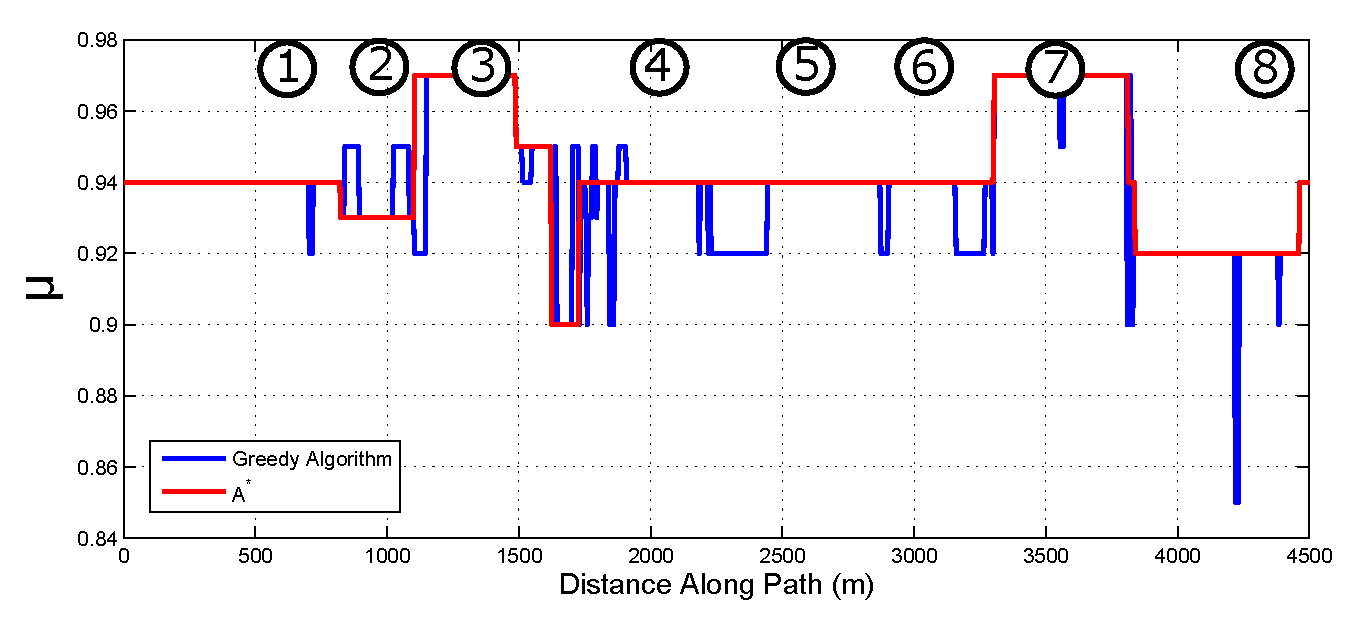
\includegraphics[width=\fullwidth]{muprofile.eps}
\caption{Minimum time $\mu(s)$ profile for Thunderhill, for both the A* solution and greedy algorithm solution.}
\label{fig:muprof}
\end{figure}  

 \begin{table}[h]
\begin{center}
\caption{Lap Times}\label{tb:predresults}
\begin{tabular}{l|c}
Driver          & Lap Time \\\hline
Constant $\mu(s)$ = 0.94 & 139.2 \\
Constant $\mu(s)$ = 0.92 & 139.4 \\
Pro Driver (Best Lap)   & 137.7\\\hline
Greedy $\mu_g(s)$ (Prediction) & 136.4 \\
A*     $\mu^*(s)$ (Prediction) & 136.8 \\\hline
\end{tabular}
\end{center}
\end{table}
 
\begin{figure}[tb]
\centering
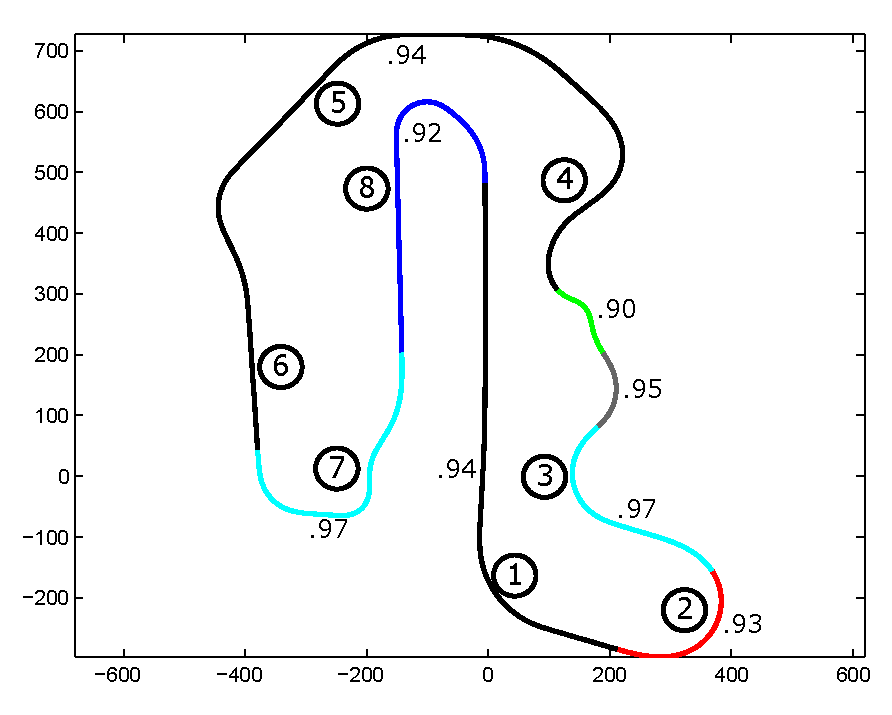
\includegraphics[width=\fullwidth]{mumap.eps}
\caption{Minimum time $\mu^\star(s)$ profile from A* algorithm plotted on map of Thunderhill.}
\label{fig:mumap}
\end{figure}  

Fig.~\ref{fig:mumap} provides interesting insights about what the A* algorithm is learning. Section \circled{2} is a 
long, sweeping turn with mostly steady-state cornering dynamics, so the optimal friction value of .93 is in the middle
of the range of possible values and representative of the average friction between the tires and the track. Sections \circled{3}
and \circled{7} represent short turns followed by a turn in the opposite direction. For these turns, the algorithm has learned it is better to drive a little
 faster than the true friction limit would dictate, because by the time the vehicle begins to understeer, the turn is already complete and
 the vehicle can reverse the steering quickly while following the desired path. Section \circled{8} occurs before a long straight section of the track where recovering
from an understeer would result in a significantly lower speed on the fastest part of the track. As a result, the algorithm's planned acceleration is more conservative. Finally, 
the section with the lowest $\mu(s)$ occurs on a part of the track with significant lateral weight transfer. In general, lateral weight transfer reduces the cornering forces available
to the vehicle, but this effect was not captured in the trajectory planning phase, which assumed a planar model with coupled left and right tires. In summary, the A*
algorithm allows the car to learn subtle but important driving behaviors that are not easily captured through simulation. 

\section{Experimental Validation}
The best validation of the A* algorithm is to experimentally drive the optimal velocity
profile $U^\star_x(s)$ generated from $\mu^\star(s)$. From Fig.~\ref{fig:muprof}, this velocity profile will have accelerations as low as 9.0 $\mathrm{m/s^2}$
on some turns, and as high as 9.7 $\mathrm{m/s}$ on others. Fig.~\ref{fig:muexpres} shows autonomous experimental data from 
driving $\mu^\star(s)$
compared to two other experiments\footnote{There was a minor change between the optimal $\mu$ profile from Fig.~\ref{fig:muprof} and what was tested experimentally. For section \circled{2}, the value of $\mu$ was set to 0.92 as opposed to 0.93. This
was a safety measure taken based on preliminary testing.}. The first experiment is a full autonomous test with a constant $\mu = 0.94$, and the second experiment is the
fastest single lap recorded by the professional race car driver in Fig.~\ref{fig:expLT}. 

\begin{figure}[tb]
\centering
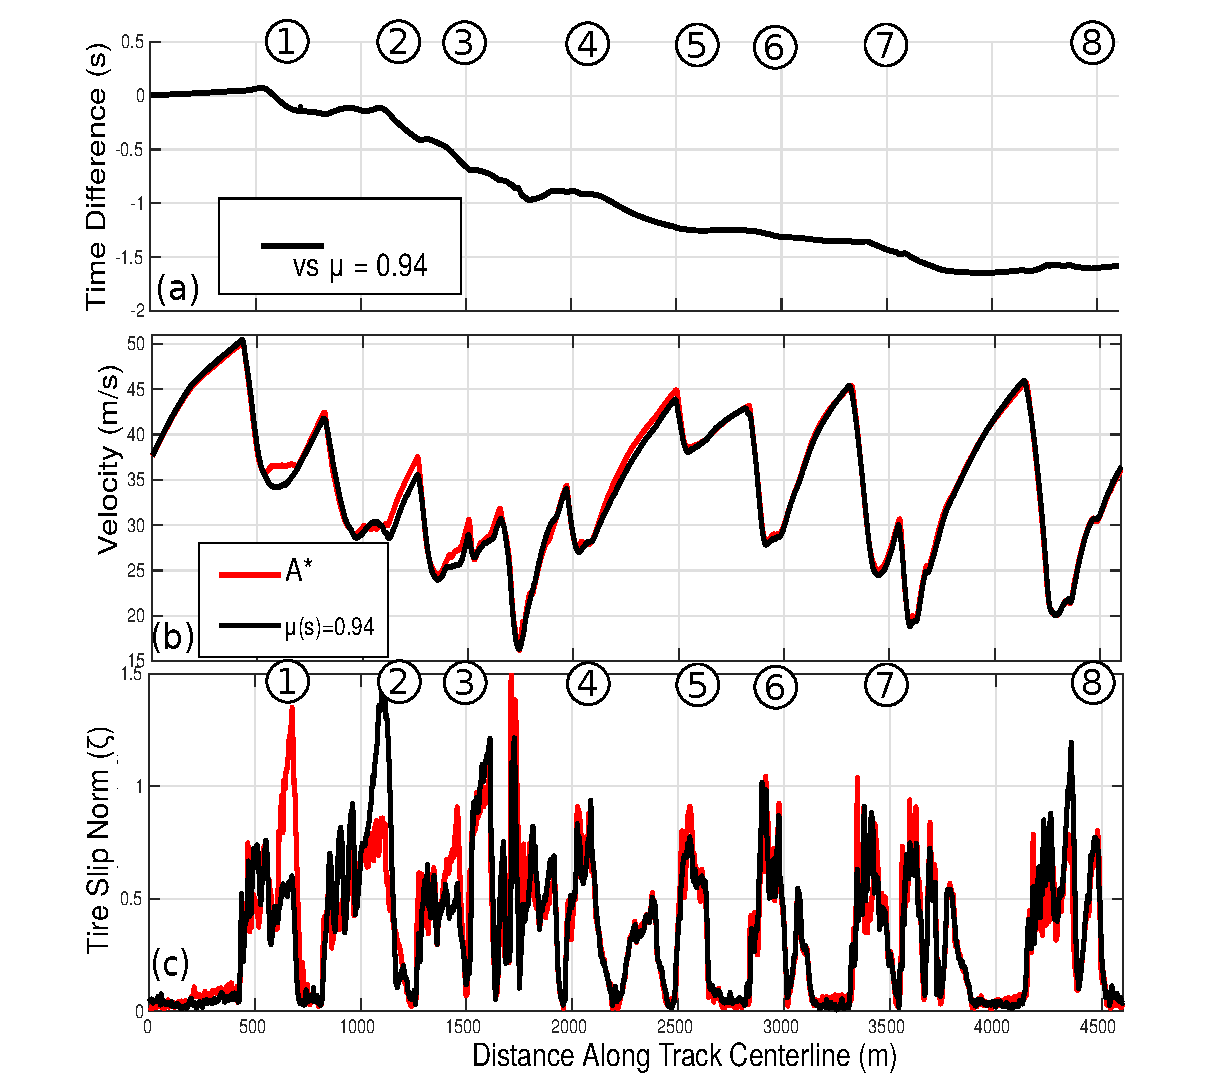
\includegraphics[width=\fullwidth]{expAstarResults.eps}
\caption[Time difference between experimental dataset collected with A* result $\mu^*(s)$ and dataset from professional driver.]{(a) Time difference between experimental dataset collected with A* result $\mu^*(s)$ and dataset from professional driver. Also
included is comparison with constant friction velocity profile at $\mu = 0.94$. Negative time distance corresponds to A* result being ahead. (b) Experimental velocities between all three experimental datasets.
(c) Tire slip norm measurements for all three datasets.}
\label{fig:muexpres}
\end{figure}  

 The experimental results show solid performance of the learned friction profile $\mu^\star(s)$. From Fig.~\ref{fig:muexpres}(a), the lap time using the learned friction
 profile is roughly 1.5 seconds faster than the lap time from the constant friction profile. The lap time is also comparable to the fastest
 recorded lap time of the pro driver. A significant part of this improved performance comes through more efficient friction usage.
 For example, in sections \circled{2} and \circled{8}, learning to drive more cautiously enables the tire slip norm $\zeta$ to drop closer to 1, avoiding
 a costly understeer. In sections \circled{3} and \circled{7}, the A* algorithm has learned that more aggressive driving is possible, increasing $\zeta$ closer to 1 and matching the tire
slip norm of the professional driver. 

However, there are several caveats associated with Fig.~\ref{fig:muexpres} to disclose. Due to time constraints, the
three datasets were all taken on different dates, meaning that weather, tire conditions, etc. were different for each test. Second,
the two autonomous datasets were taken nearly a year apart, and as a result, there were independent improvements made to the vehicle controllers
that also contribute to the 1.5 second experimental lap time improvement. For example, the higher speed in section \circled{1} (see Fig.~\ref{fig:muexpres}(a))
was due to a more tightly tuned longitudinal controller and not a difference in the desired speed profile. Finally, because autonomous racing is performed with nobody in the vehicle, 
the human driver has the disadvantage of both his added mass and the added mass of a graduate student. Since
the available engine force is limited, this decreases the available acceleration on straight sections of the track by roughly 10\%. 
This gives a time boost for any autonomous lap over a human-driving lap, as seen by the higher top speeds in Fig.~\ref{fig:muexpres}(b).
 

\section{Future Work}

There are a several next steps to improve the preliminary research presented in this chapter. First, the algorithm presented here assumes
the availability of pre-existing data. For a track where existing data at the handling limits is unavailable, the algorithm should be modified
so that laps are driven at a low assumed friction value (i.e. $\mu$ = 0.9) and slowly ramped up, with the A* algorithm used after
every lap to find portions on the track where the vehicle could benefit from a more aggressive acceleration profile. 

Finally, the algorithm makes the key assumption that observations made on prior laps will hold for upcoming laps. However, when data is collected for the same
velocity profile multiple times, the resulting observed speeds and tire slips will vary. Furthermore, the tire slip norm $\zeta$, defined in Chapter 4,
is a noisy empirical estimate of whether the vehicle is actually sliding. Further
work is necessary to add uncertainty to the model. For example, preliminary work is underway to treat experimental tire slip measurements as noisy
indicators of whether the vehicle has exceeded the limits. This would complement the existing literature for real-time vehicle decision making under uncertainty, which
has considered uncertainty in sensor noise, perception constraints, and the behavior of surrounding vehicles and pedestrians \cite{brechtel}\cite{ulbrich}\cite{wei}. Accounting for state uncertainty by developing a Partially Observable Markov Decision Process (POMDP)
is therefore a promising avenue for future work. 

\newpage
\section{Conclusion}

This chapter presented an algorithm to improve the experimental lap time of an autonomous race car by learning the optimal friction
profile, and therefore the optimal desired speed and acceleration profiles. The approach works by searching through a tree
built up from experimentally collected observations and finding the fastest speed profile via an A* implementation. Edge costs
for this tree are given by travel time calculations and a switching cost that accounts for the difficulty of speed control while the
vehicle is understeering or oversteering. The results compared well experimentally to an autonomous dataset 
from a uniform $\mu$ profile and against an experimentally recorded dataset from a professional driver.

The significance of this work is that the autonomous race vehicle is no longer required to race with a single predetermined estimate of
the tire-road friction. Experimental data indicates that in reality, each turn on the track has a slightly different acceleration limit 
that enables the autonomous vehicle to minimize travel time without sliding off the track. Instead of naively guessing an average
friction/acceleration limit for the entire racing circuit, the presented algorithm allows the vehicle to search through data obtained from previous laps and find an
optimal friction \textit{profile} that varies along the track.

